\subsection{Product perspective}

SafeStreets is built from the ground up as a new software application, specifically a mobile application, as required by the functionality that is provided. This mobile app communicates with a server, where the data is analysed and stored. External services are also utilized, particularly a government licence plate registry and a maps API.

As for the SafeStreets system, the domain model is described in the diagram shown in Figure~\ref{fig:class-general}. Note that the diagram is not a complete description of the system, but rather a simplified version for easier understanding.

\begin{figure}[!h]
\centering
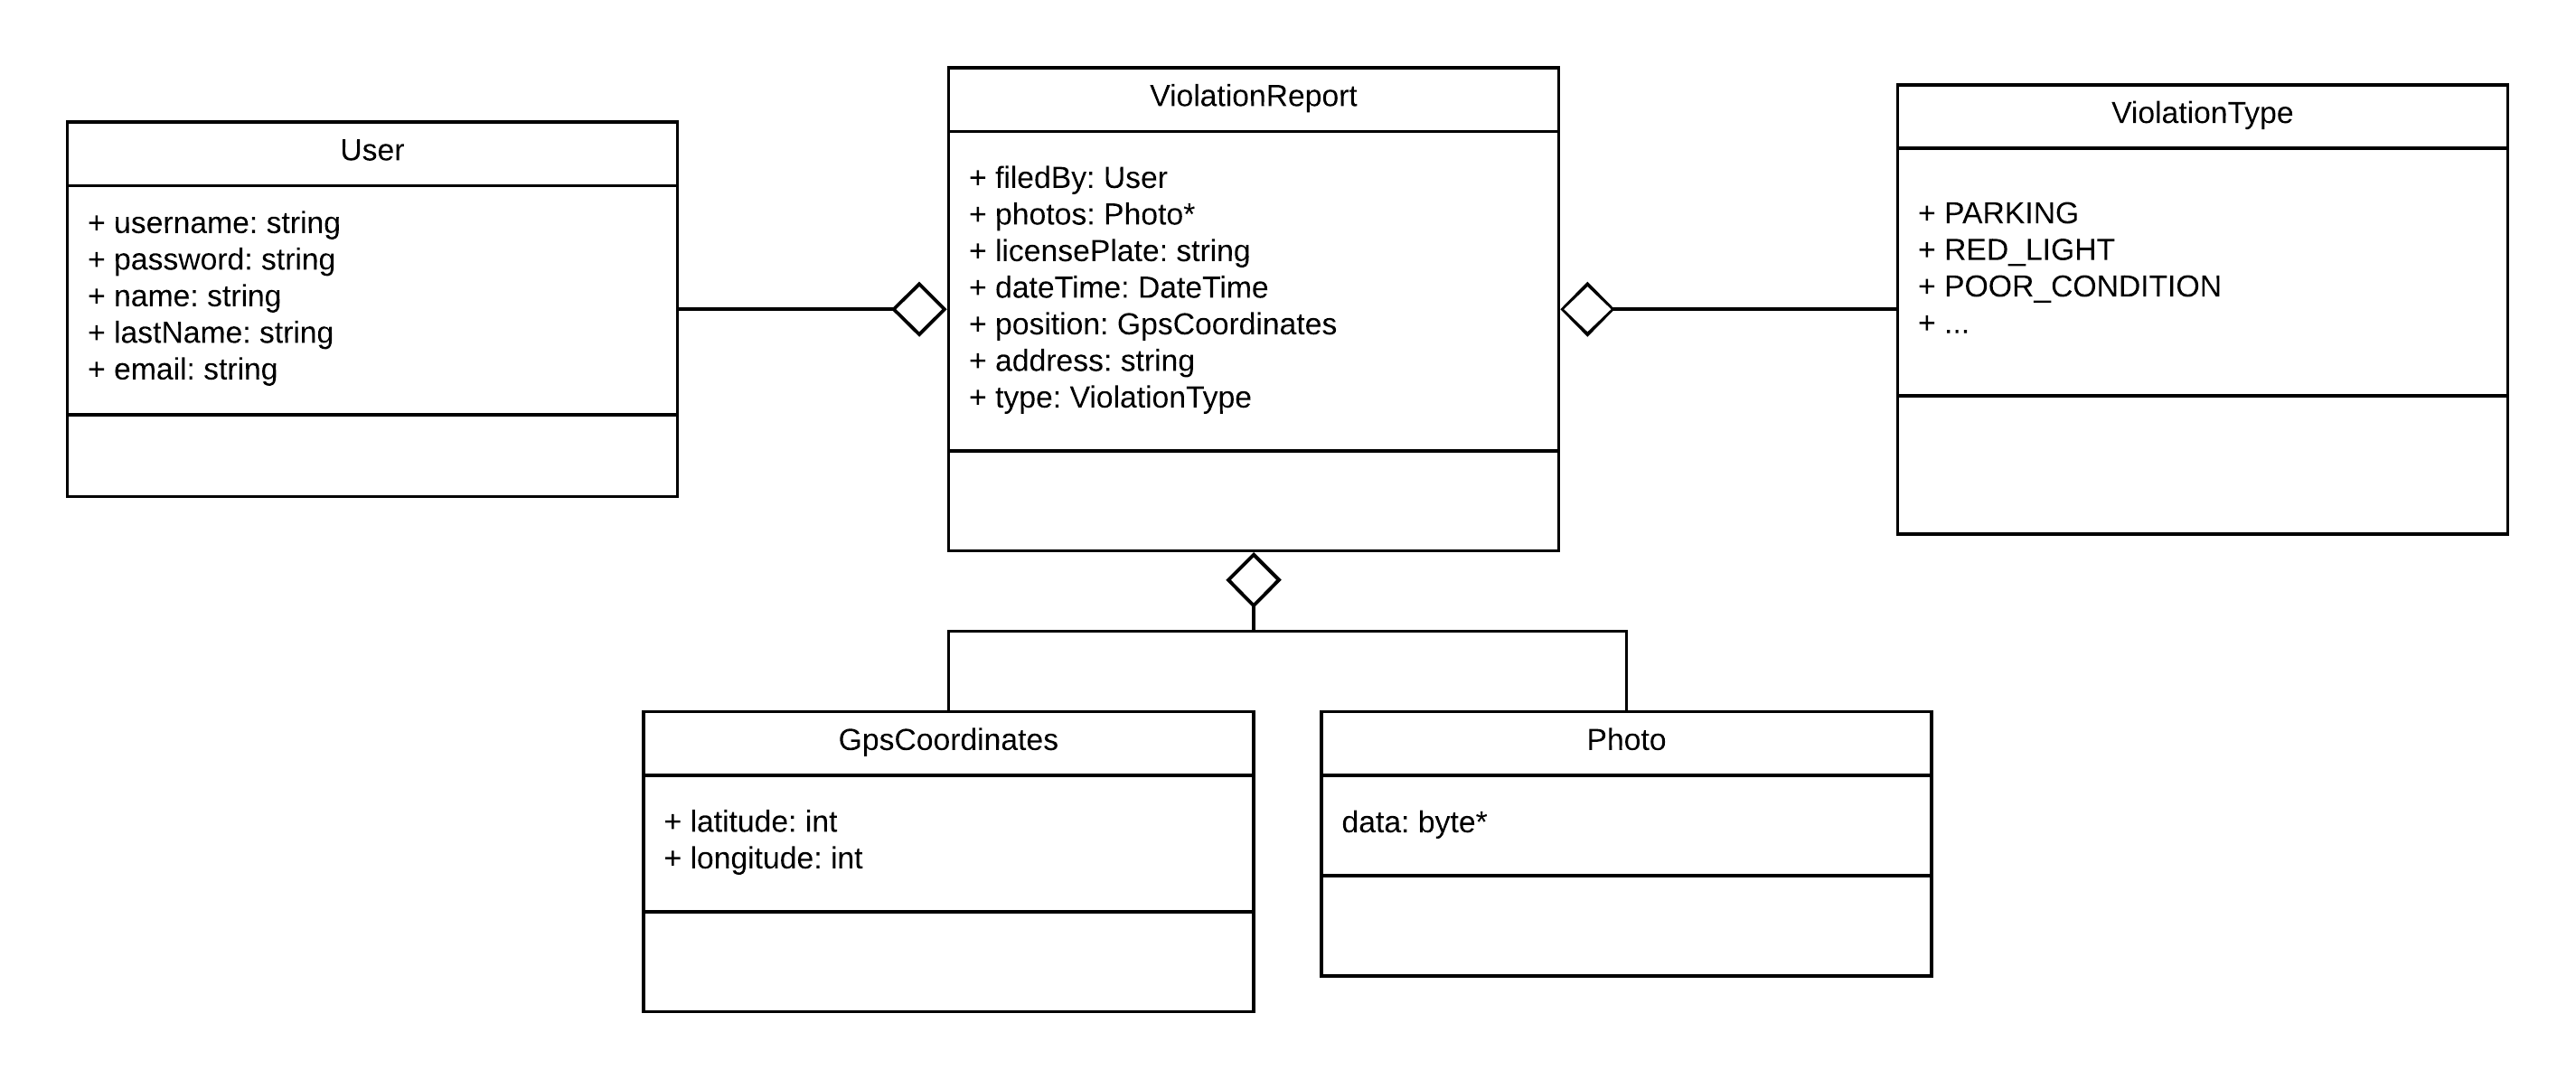
\includegraphics[width=\textwidth]{Images/class-general.png}
\caption{\label{fig:class-general}Class diagram.}
\end{figure}

Inspecting the class diagram, we can see that most of the system revolves around the violation reports and their processing, as this is the core functionality of the system.
In the state diagram shown in Figure~\ref{fig:state-report-submission}, the process of submitting a report is explained.

\begin{figure}[!h]
\centering
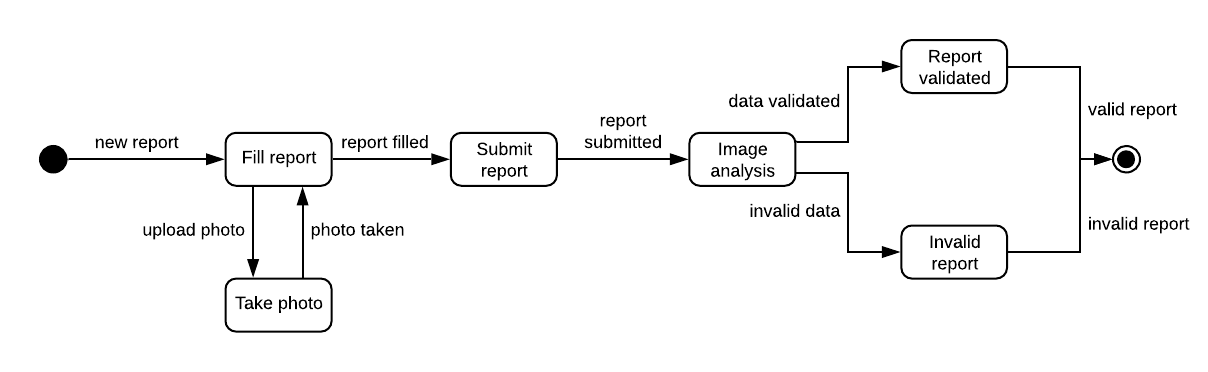
\includegraphics[width=\textwidth]{Images/state-report-submission.png}
\caption{\label{fig:state-report-submission}State diagram - Report submission.}
\end{figure}

As observed there, for submitting a report, the user is required to both fill a form with the required information and take photos of the event. After the submission, the SafeStreets system executes an analysis of the data, matching it with the provided image. This can result in either an invalid or a valid report. A valid report is saved and made available for the different users to query, either through the mobile application or through the public API. Invalid reports are still kept to be analyzed and detect any problems with the system, but are not shown to regular users nor authorities.

Further explaining the analysis process Figure~\ref{fig:state-report-validation}, the system utilizes a license plate recognition algorithm of which the output consists of possibly multiple license plates (the picture could include more than one car), along with the certainty of the detection.
The target of the report is determined by comparing the detections with the license plate manually submitted by the user.

\begin{figure}[!h]
\centering
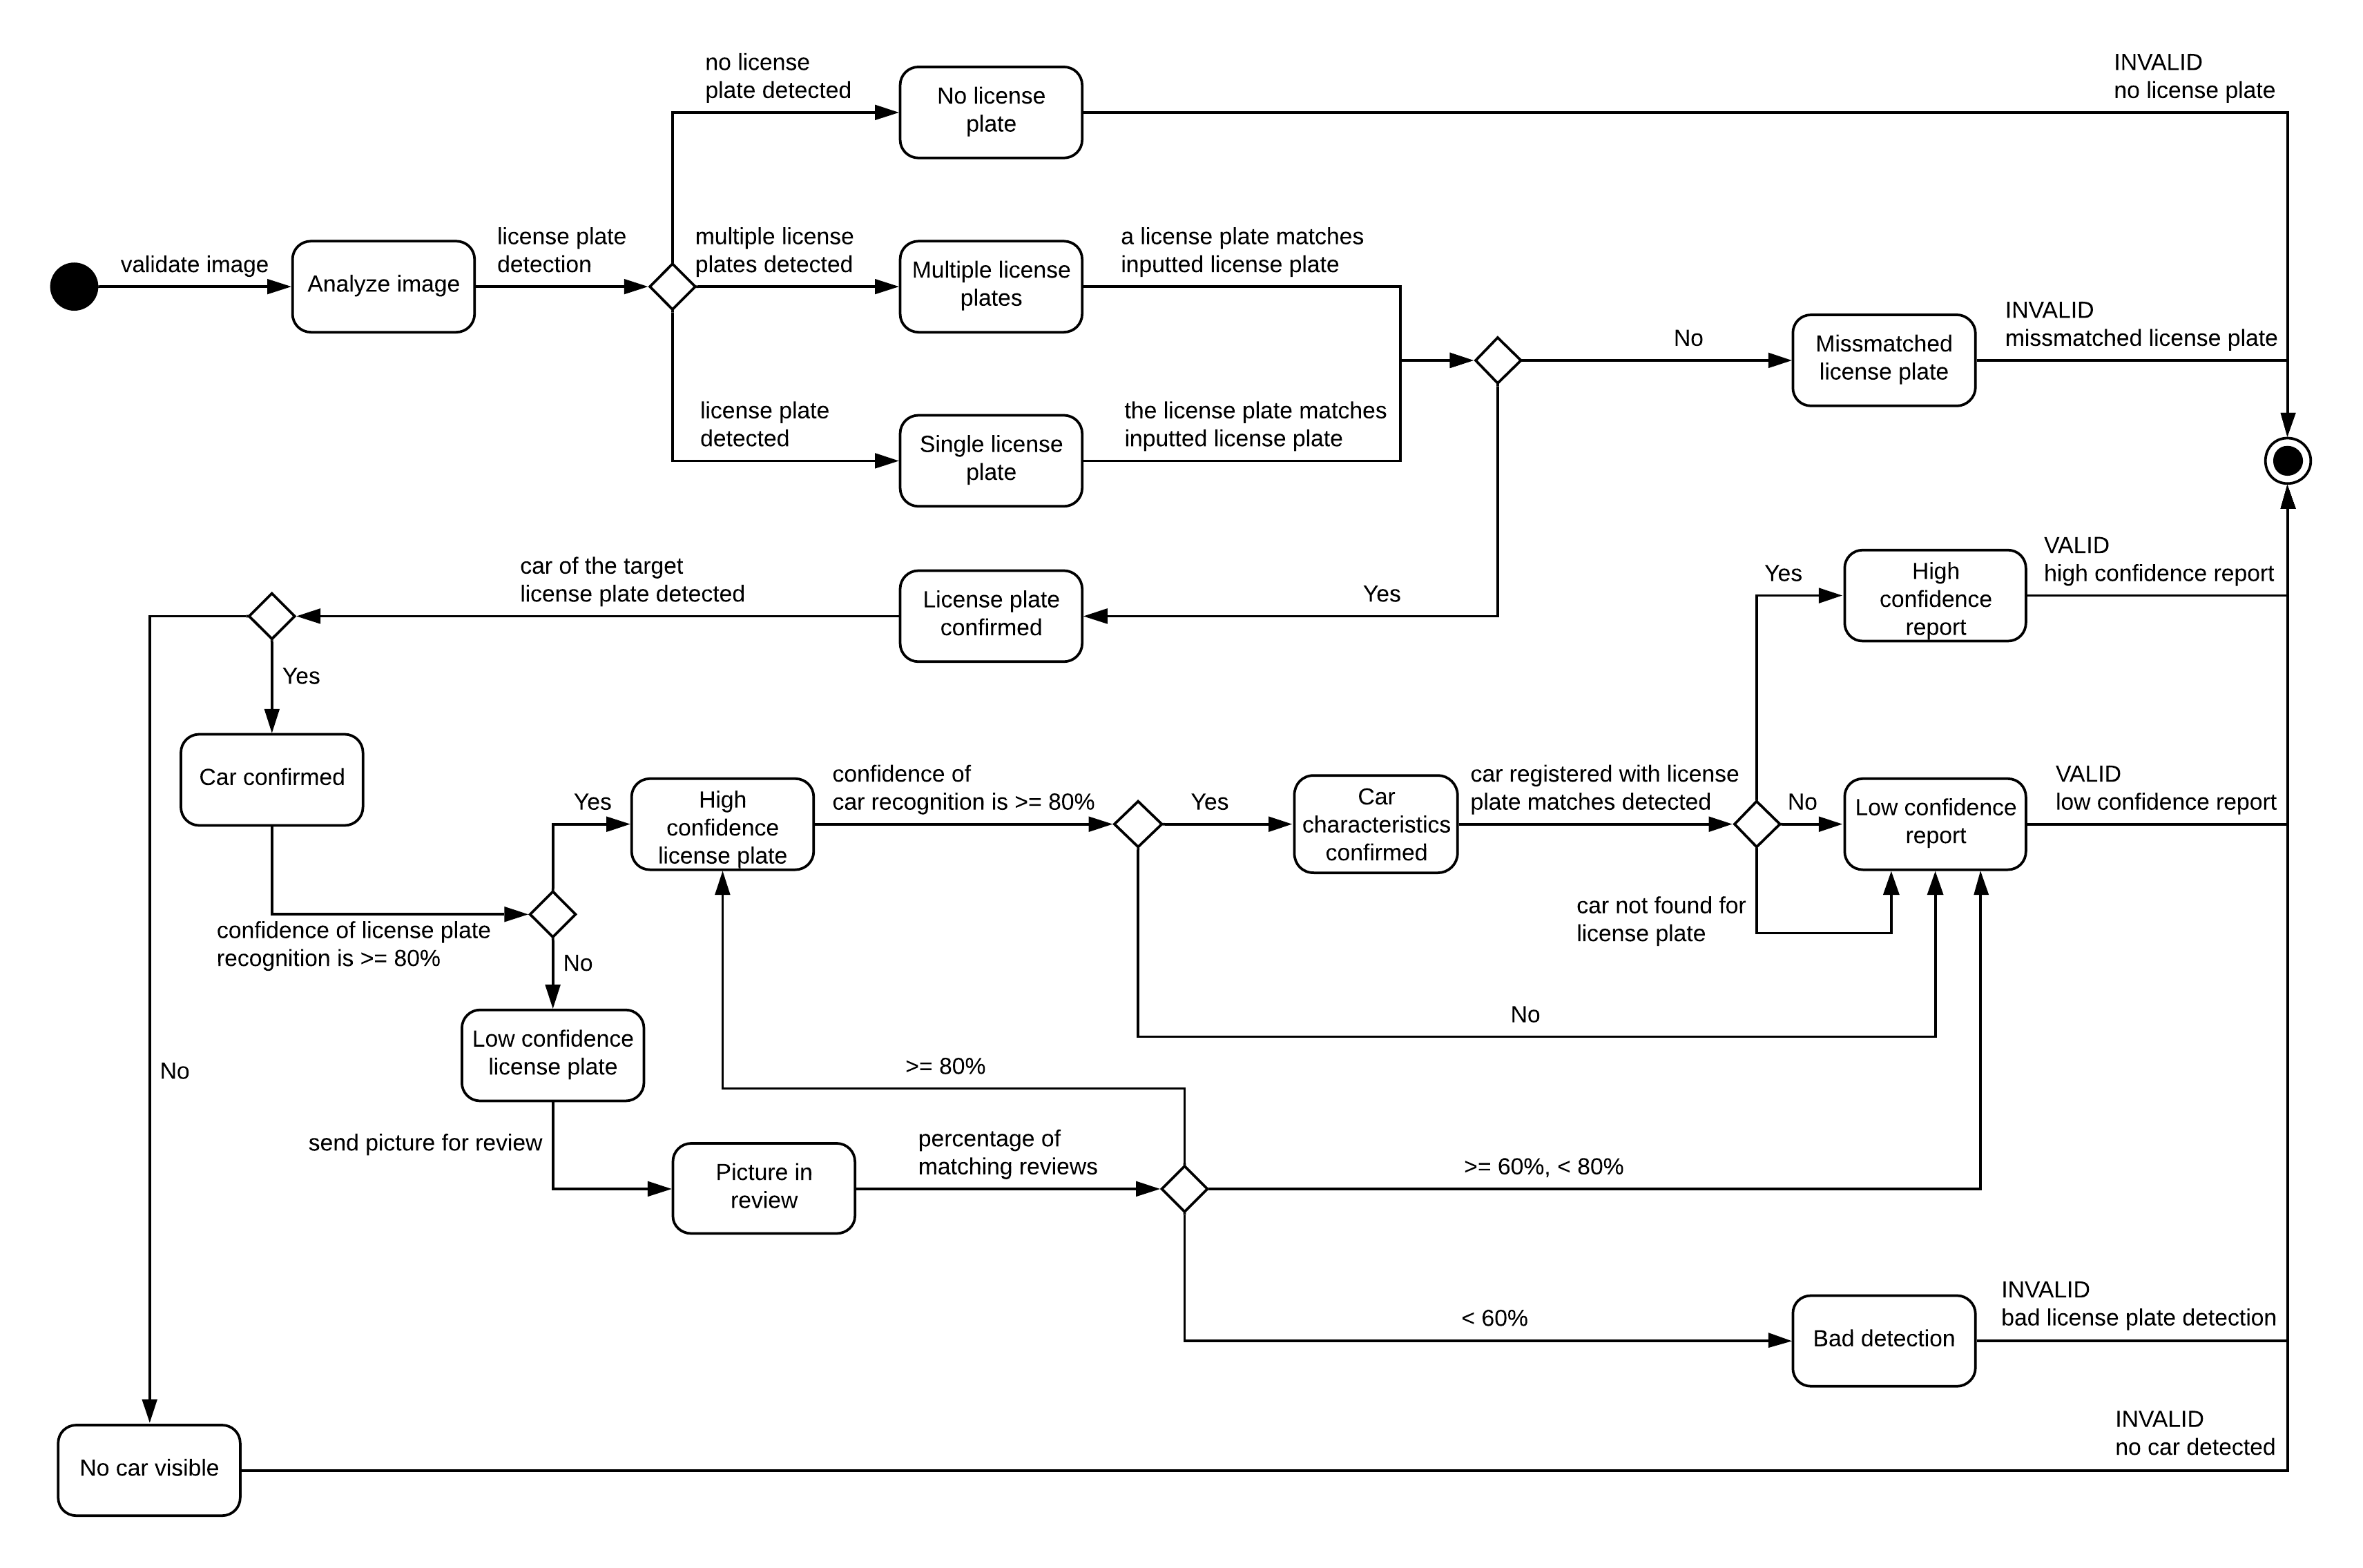
\includegraphics[angle=-90,origin=c,width=\textwidth]{Images/state-image-validation.png}
\caption{\label{fig:state-report-validation}State diagram - Image validation.}
\end{figure}

After the target license plate is confirmed, the confidence of the detection is evaluated, if it is below a certain threshold, it must pass through a community review. During this process, multiple users willing to participate are shown a cutout of the license plate in the picture and asked to input what they see. If a consensus is reached, then the report is considered valid.

A valid report is then checked for good car recognition and that the detected car and license plate match with the local license plate registry. If these checks pass, the system is confident enough that authorities could issue a proper traffic ticket based on the report.

Users can access data provided by the system through both the mobile application and the public API. In the second case, as seen in Figure~\ref{fig:api-usage}, the process is fairly simple. Here, the user asks for reports matching the filters and provides their api key for authentication. The key can be obtained through the application by standard users and its provided by an administrator in the case of authorities. The system uses this key to check if the user has the required permissions to access the data requested.

\begin{figure}[!h]
\centering
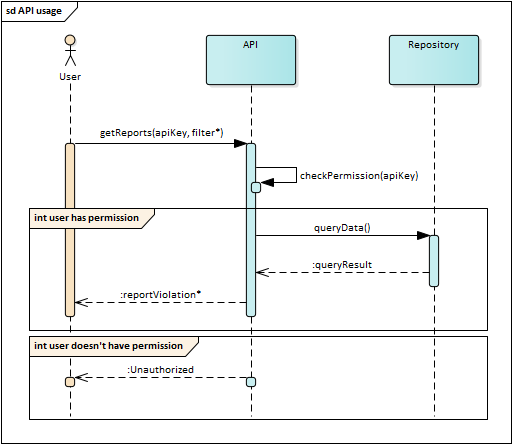
\includegraphics[width=\textwidth]{Images/api-usage.png}
\caption{\label{fig:api-usage}Sequence diagram - API Usage.}
\end{figure}

\subsection{Product functions}
The functionality of the system can be divided into three groups. In the following section, these functions are listed and explained, taking into account the already specified goals of the system.

\subsubsection{Violation report}
The reporting of violations is the main functionality of the system. It allows its registered users to submit a traffic violation report. The user is required to provide data, such as pictures of the violation, the license plate of the vehicle committing the violation and the type of violation. On top of this information, the mobile application will provide the system with metadata which includes the gps location, date and time of the report.
After the submission, the system analyses the provided information, checking its integrity. A valid report is shared with the users, and an invalid report is hidden but available internally for analysis and troubleshooting.

\subsubsection{Image analysis}
In order to confirm the validity of a report, the system performs an analysis of the submitted images. The pictures are expected to show the vehicle committing the violation, with at least one of them providing a clear view of its license plate. The analysis searches the images for this information and matches the detected license plate with the one provided by the user in the report. If the analysis is not certain enough, the system gets support from its users by showing them the photo and asking them to input the license plate being shown.

\subsubsection{Data querying}

Gathered information by SafeStreets can be accessed by all users. There are two ways in which the data can be accessed, via the mobile application or through the public API.

In the first case, the mobile application provides users with the ability to see violations in a map, allowing the user to also filter these violations by date and type. 
On the other hand, the API allows for SafeStreets to be integrated with other third party systems. Users are able to query the available data according to their role and obtain the information in an analysis-friendly format.

The data provided for each violation is the following:
\begin{itemize}
\item Report ID: unique reference to each report
\item Type of violation
\item Date and time
\item Location: gps coordinates, approximate street name and number
\item Photos
\item License plate
\item The system’s degree of confidence in the report
\item Whether the report contributed to issuing a traffic ticket
\end{itemize}


\subsection{User characteristics}
The actors identified as the users of the application are:
\begin{itemize}
\item
User: Also referred to as the “standard user”. A person that has registered to SafeStreets and is capable of reporting violations, seeing the reports map and reviewing photos. 
\item
Municipality system: A system belonging to the municipality that communicates with SafeStreets through the exposed API. Capable of accessing more information than the standard user.
\item
Administrator: An employee of SafeStreets that maintains and updates the system.
\end{itemize}

\subsection{Assumptions, dependencies and constraints}

\begin{itemize}[label={}]
    \item \begin{assumption} Location obtained from the device running SafeStreets is accurate. \end{assumption}
    \item \begin{assumption} Date and time obtained from the device running SafeStreets is accurate. \end{assumption}
    \item \begin{assumption} The information provided by the ticketing system is accurate and up to date. \end{assumption}
    \item \begin{assumption} The information provided by the license plate registry is accurate and up to date. \end{assumption}
\end{itemize}